\documentclass{article}
\usepackage{graphicx}
\usepackage{wrapfig}
\usepackage{filecontents}
\usepackage{siunitx}
\usepackage[table]{xcolor}
\usepackage{float}
\usepackage{hyperref}

\usepackage{color} % balíček pro obarvování textů
\usepackage{xcolor}  % zapne možnost používání barev, mj. pro \definecolor
\usepackage{pgfplots} % http://www.chiark.greenend.org.uk/doc/texlive-doc/latex/pgfplots/pgfplots.pdf

\ifnum 0\ifxetex 1\fi\ifluatex 1\fi=0 % if pdftex
  \usepackage[T1]{fontenc}
  \usepackage[utf8]{inputenc}
\else % if luatex or xelatex
  \ifxetex
    \usepackage{mathspec}
  \else
    \usepackage{fontspec}
  \fi
  \defaultfontfeatures{Ligatures=TeX,Scale=MatchLowercase}
\fi
\usepackage[total={175mm,230mm}, top=23mm, left=20mm, includefoot]{geometry}
\hypersetup{
    colorlinks,
    linkcolor={blue!50!black},
    citecolor={green!50!black},
    urlcolor={blue!80!black}
}
\definecolor{orange}{RGB}{ 251, 114, 032}
\definecolor{fialova}{RGB}{ 255, 000, 255}

\newcounter{obrazky}
\setcounter{obrazky}{1}
\newcommand \obrlabel[1]
{ 
  obr.~\theobrazky
  \stepcounter{obrazky}
  \label{#1}
}


\newcommand \obr[1]
{ obr.~\ref{#1}}

\newcommand \tab[1]
{ tab.~\ref{#1}}


\begin{document}
Tomáš Vavrinec \- \- \- 240893

\section{Nízkofrekvenční zesilovače s OZ}
\subsection*{Střídavý zesilovač s nesymetrickým napájením operačního zesilovače}
\begin{figure}[H]
  \begin{minipage}[t]{0.48\textwidth}
    \vspace{10mm}
    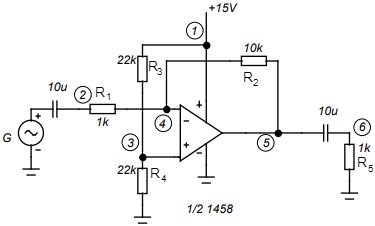
\includegraphics[width=\textwidth]{uvod/posun.png}
  \end{minipage}
  \hfill
  \begin{minipage}[t]{0.48\textwidth}
    % \vspace{-50mm}
    Abychom si vystačili s jedním zdrojem vytvoříme referenční napětí pro neinvertující vstup.

    \subsection{DC}
      Na vstupu je kondenzátor a do vstupu OZ neteče žádný proud \(\Rightarrow\) skrz \(R_1\) a \(R_2\) neteče žádný proud.
      V uzlech \(2, 4, 5\) a \(3\) je tedy stejné napětí a to \(U\frac{R_4}{R_4 + R_3} = \Left(15\frac{22\cdot10^{3}}{22\cdot10^{3}+22\cdot10^{3}} \Right) \-[V]= 7.5\-[V]\)
    \subsection{AC} 
      Na vstup přivedeme \(1\-[V]\) s frekvencí \(1\-[kHz]\)
      \(
        U_{5} = -\frac{R_2}{R_1} U_{vst} = -\frac{10\cdot10^{3}}{1\cdot10^{3}} \cdot 1 = -10\-[V]
      \)    
  \end{minipage}
\end{figure}

\subsection*{Sumační zesilovač}
\begin{figure}[H]
  \begin{minipage}[t]{0.48\textwidth}
    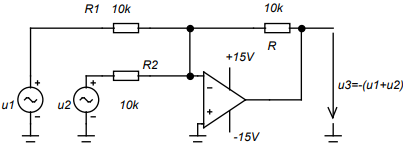
\includegraphics[width=\textwidth]{uvod/sou.png}
  \end{minipage}
  \hfill
  \begin{minipage}[t]{0.48\textwidth}
    \vspace{-20mm}
    \(
      U_{1} = 0\-[V] \Rightarrow I_{R1} = \frac{U_1}{R_1} ; I_{R1} = \frac{U_2}{R_2}

      I_{R3} = I_{R1} + I_{R2} \Rightarrow U_3 = R_3 I_{R3} = R_3\left(\frac{U_1}{R_1} + \frac{U_2}{R_2}\right) \\ U_3 = \frac{R_3}{R_1} U_1 + \frac{R_3}{R_2} U_2
    \)
  \end{minipage}
\end{figure}

\subsection*{Diferenční zesilovač}
\begin{figure}[H]
  \begin{minipage}[t]{0.48\textwidth}
    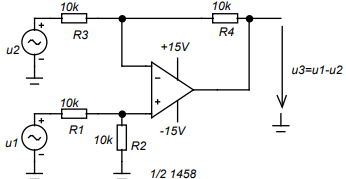
\includegraphics[width=\textwidth]{uvod/odc.png}
  \end{minipage}
  \hfill
  \begin{minipage}[t]{0.48\textwidth}
    \vspace{-35mm}
    \(
      U_{BA} = 0\-[V] \Rightarrow U_A = U_B = U_1 \frac{R_2}{R_2+R_1}

      I_{R3} = I_{R4} = \frac{U_2-U_A}{R_3} = \frac{U_2-U_1\frac{R_2}{R_2+R_1}}{R_3}

      U_3 = U_A - I_{R4}R_4 = U_1 \frac{R_2}{R_2+R_1} - \frac{U_2-U_1\frac{R_2}{R_2+R_1}}{R_3}R_4
    \)
  \end{minipage}
\end{figure}




\section*{Simulace}
\subsection*{Střídavý zesilovač s nesymetrickým napájením operačního zesilovače}
\begin{figure}[H]
  \begin{minipage}[t]{\textwidth}
    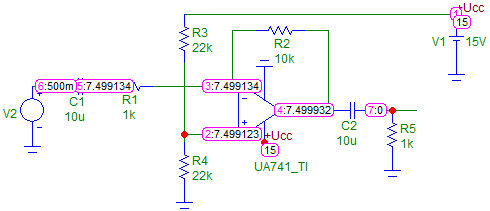
\includegraphics[width=\textwidth]{PC/ukol1/DC.png}
  \end{minipage}
\end{figure}

\begin{table}[H]
  \centering
  \begin{tabular}{|c|c|c|c|c|c|c|} 
    \hline
    uzel \(n\)          & 1       & 2      & 3     & 4     & 5       & 6      \\ \hline
    DC \(U_{nG}\-[V]\)  & 15.074  & 7.536  & 7.539 & 7.536 & 7.537   & 0      \\ \hline
    AC \(U_{nG}\-[mV]\) & 4.800   & 67.307 & 2.327 & 2.894 & 659.685 & 656.3  \\ \hline
  \end{tabular}
  \normalsize
  \caption{\label{tab_pracovni_bod_rozladeni1} Napětí v uzlech zaměřené na LC (čísla uzlu dle schematu v zadání)}
\end{table}

\begin{figure}[H]
  \vspace{-5mm}
  \begin{minipage}[t]{\textwidth}
    \centering
    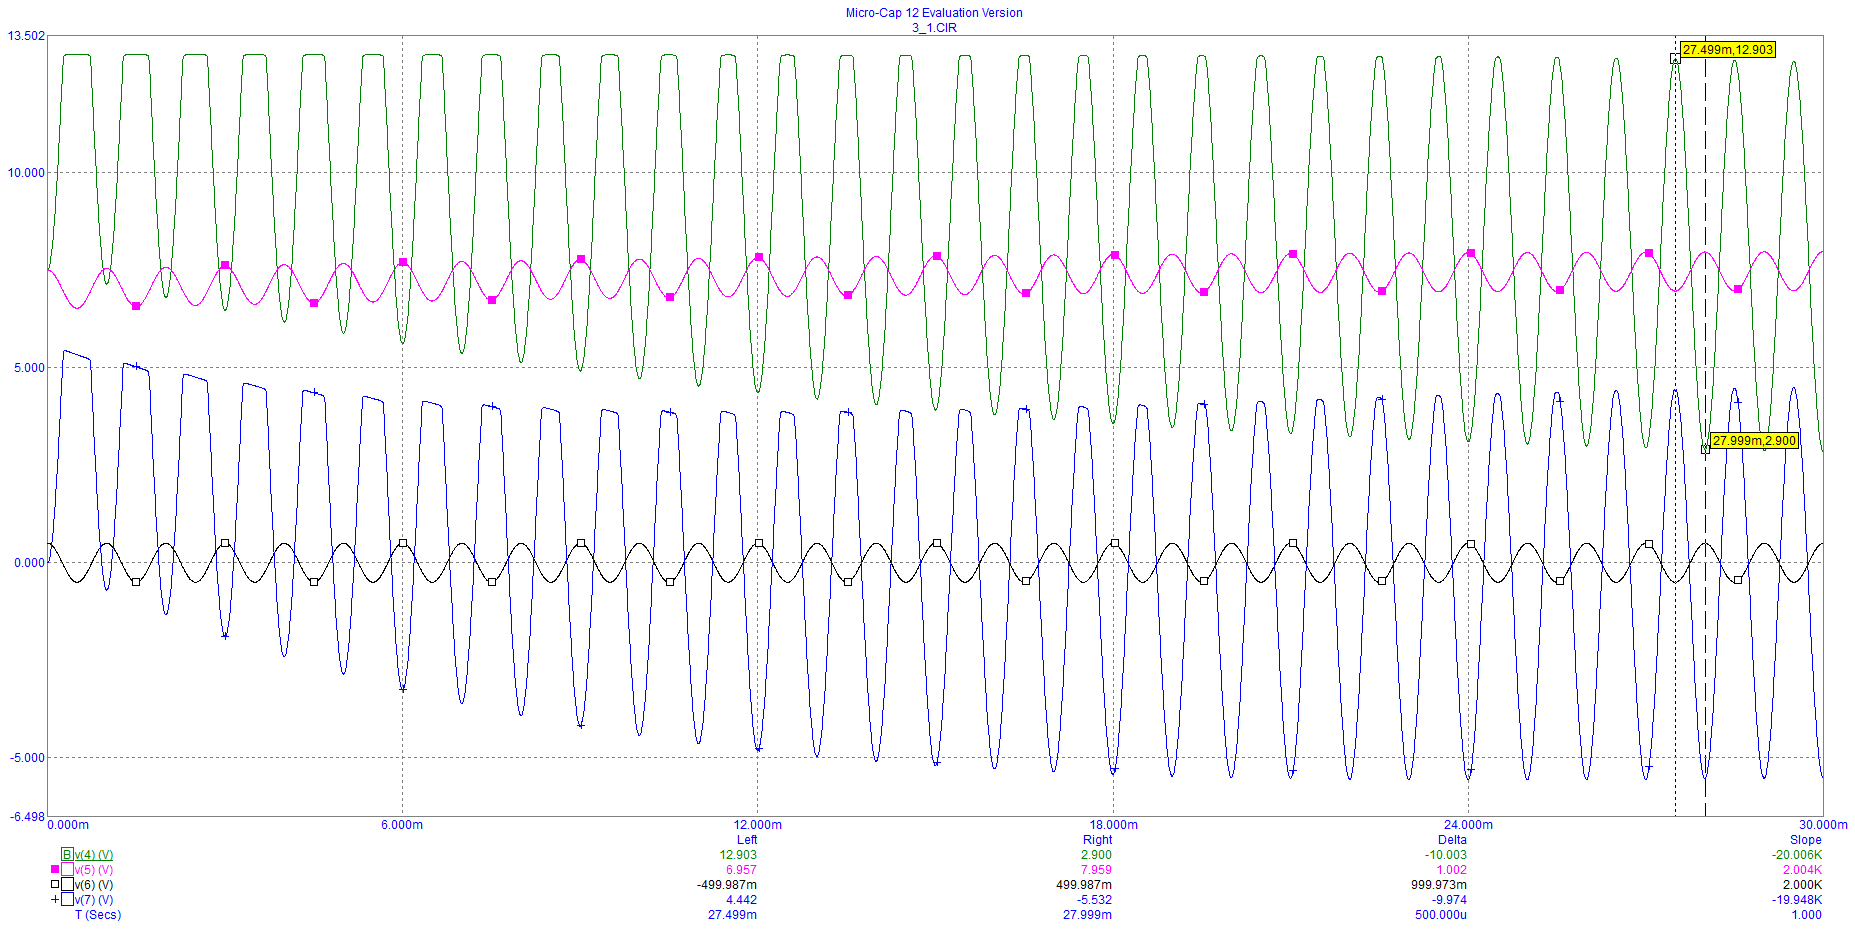
\includegraphics[width=\textwidth]{PC/ukol1/transient.png}
    Časový průběh s vyznačenými maximy na výstupu OZ.
  \end{minipage}
\end{figure}

\begin{figure}[H]
  \begin{minipage}[t]{\textwidth}
    \centering
    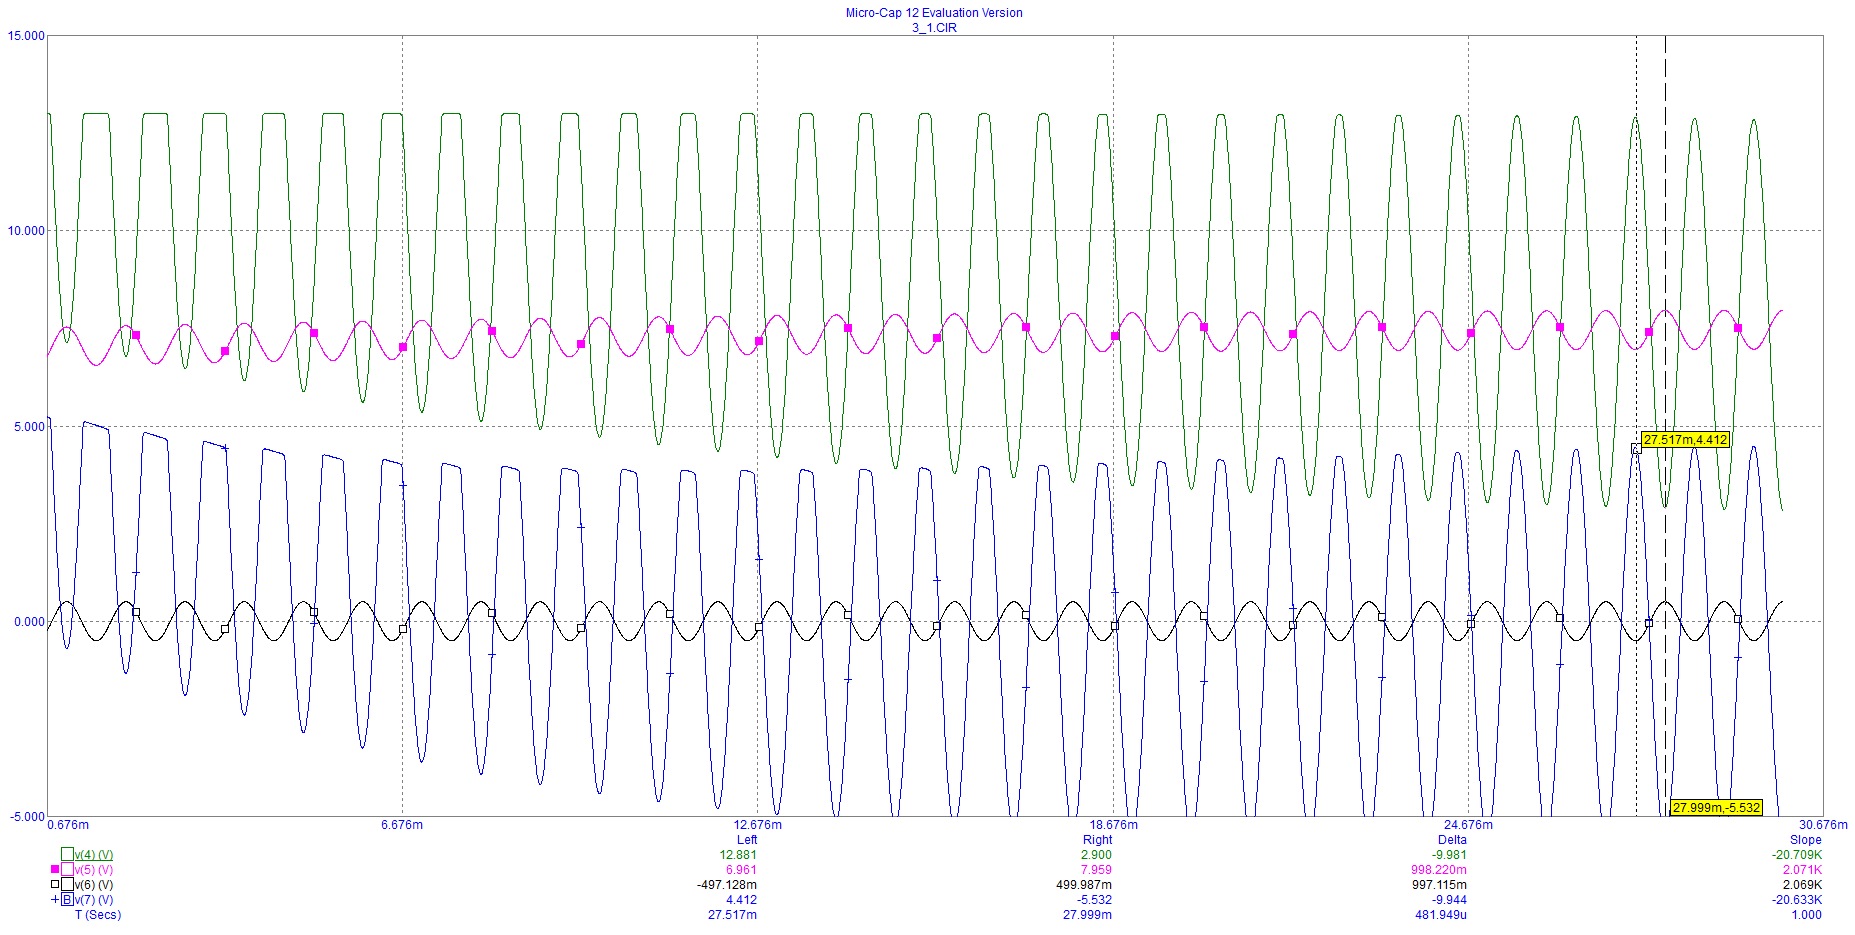
\includegraphics[width=\textwidth]{PC/ukol1/transient7.png}
    Časový průběh s vyznačenými maximy na výstupu zapojení.
  \end{minipage}
\end{figure}

\begin{figure}[H]
  \begin{minipage}[t]{\textwidth}
    \centering
    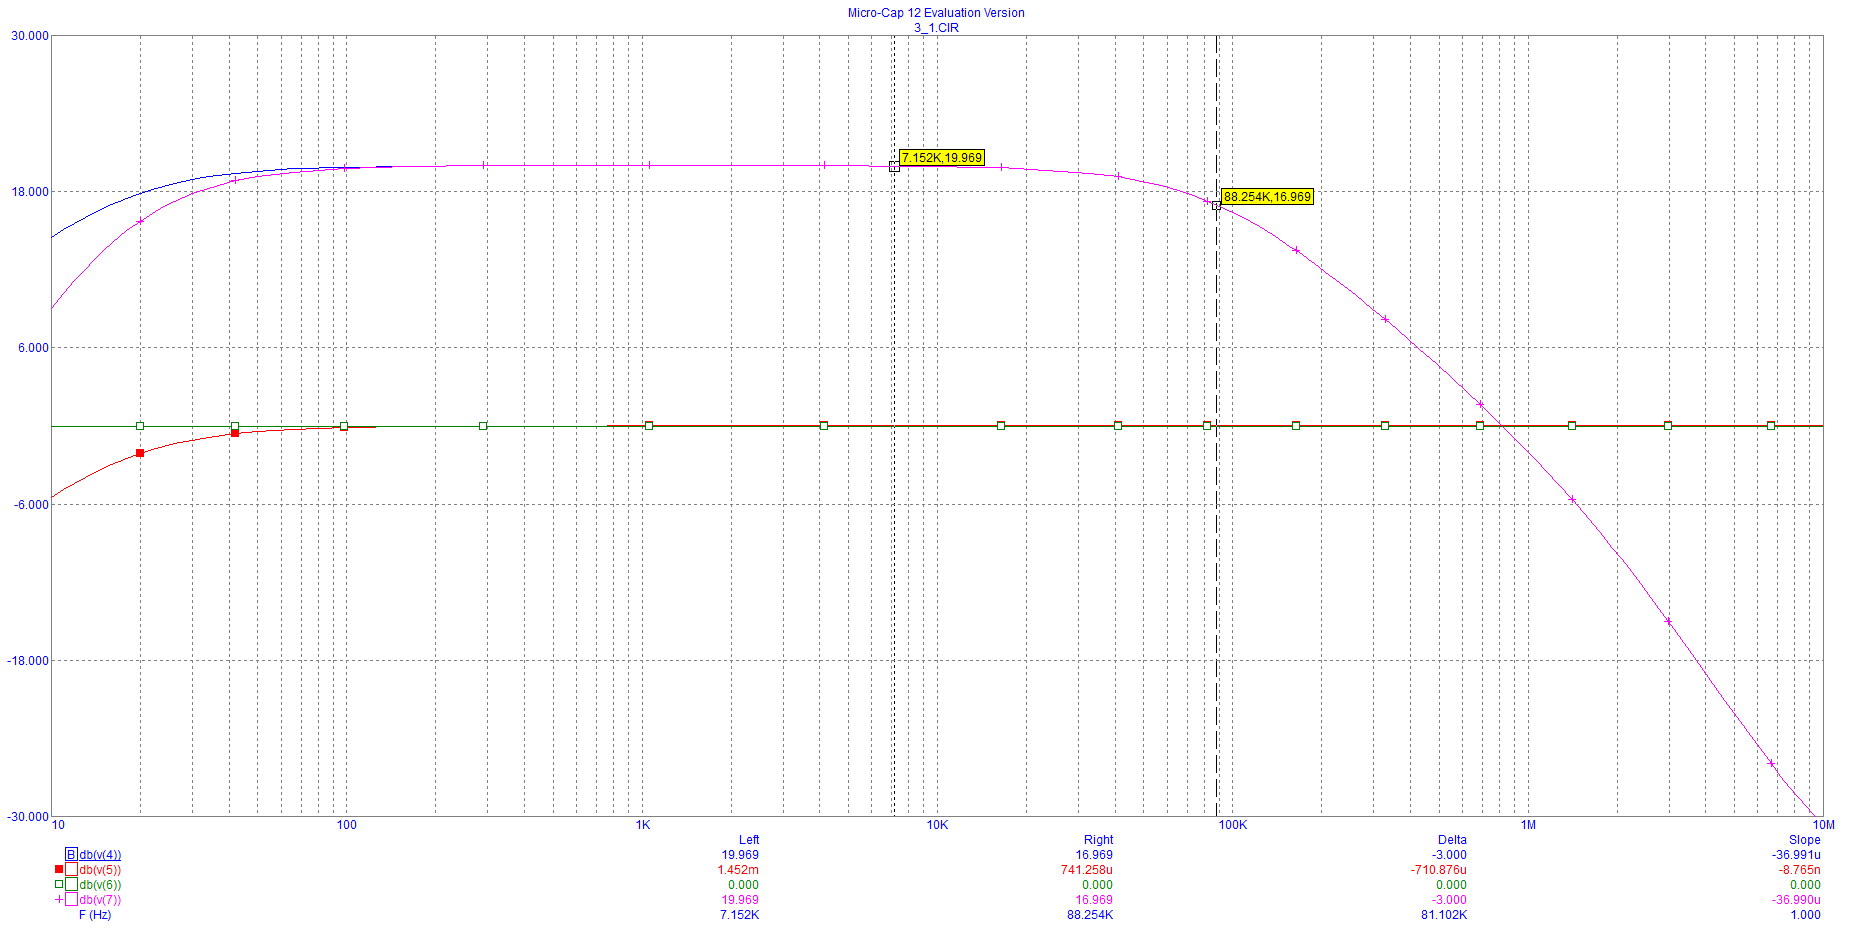
\includegraphics[width=\textwidth]{PC/ukol1/AC2.png}
    Amplitudová kmitočtová charakteristika.
  \end{minipage}
\end{figure}

\begin{figure}[H]
  \begin{minipage}[t]{\textwidth}
    \centering
    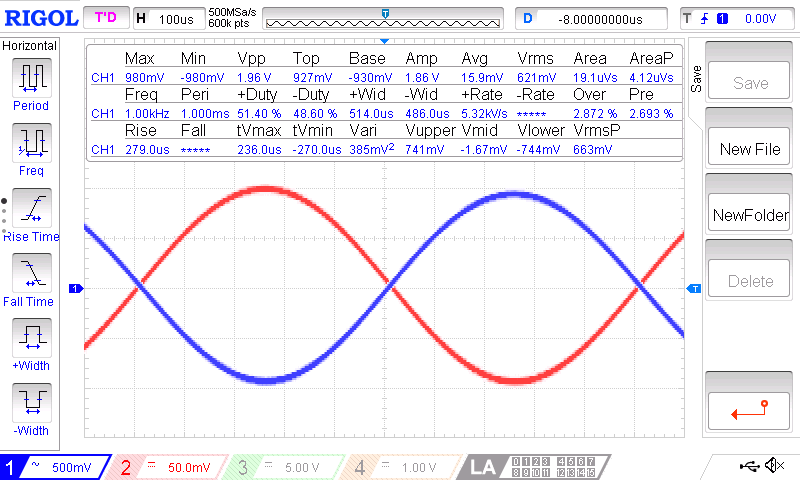
\includegraphics[width=\textwidth]{LAB/NewFile2.png}
    Změřený časový průběh, zesílení \(-10\).
  \end{minipage}
\end{figure}

\subsection*{Sumační zesilovač}
\begin{figure}[H]
  \begin{minipage}[t]{\textwidth}
    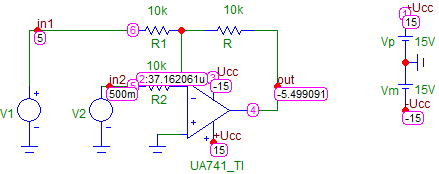
\includegraphics[width=\textwidth]{PC/ukol2/DC.png}
  \end{minipage}
\end{figure}

\begin{figure}[H]
  \begin{minipage}[t]{\textwidth}
    \centering
    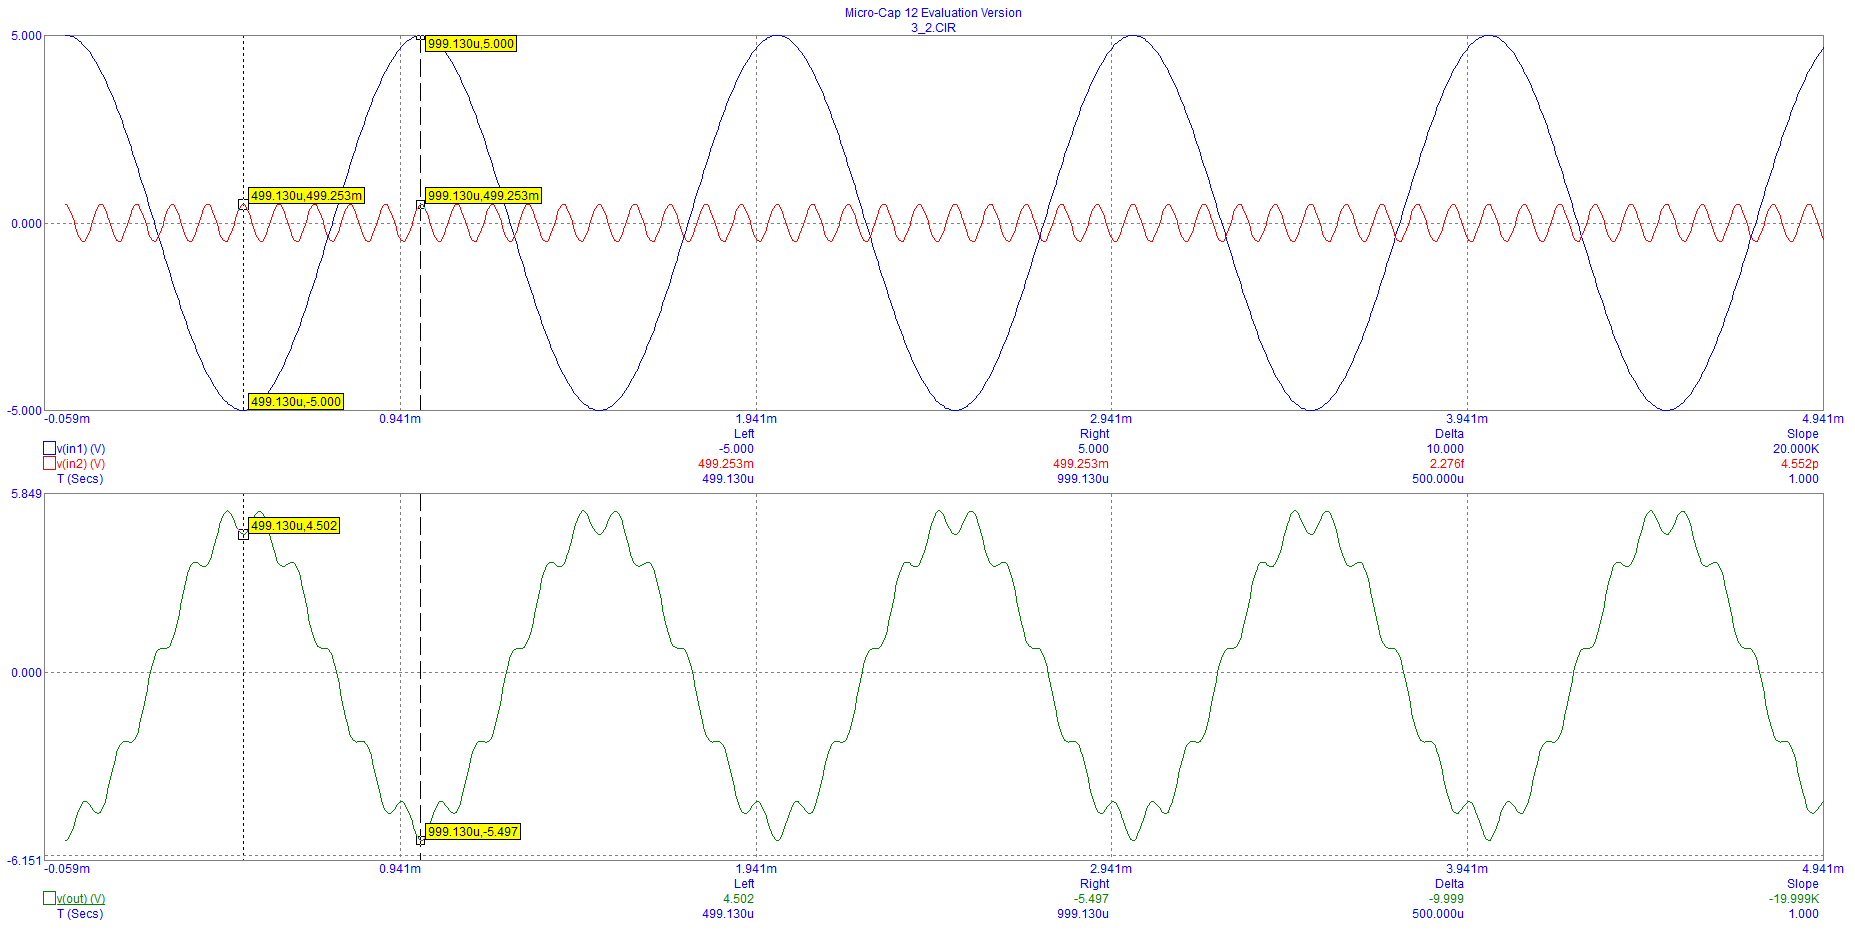
\includegraphics[width=\textwidth]{PC/ukol2/transient2.png}
    Časový průběh dvou různých signálů sumačním zesilovače a jeho výstup.\\
    signál-1 \(U_{pp} = 10\-[V]\) \(f = 1\-[kHz]\)\\
    signál-2 \(U_{pp} = 1\-[V]\) \(f = 10\-[kHz]\)
  \end{minipage}
\end{figure}

\begin{figure}[H]
  \begin{minipage}[t]{\textwidth}
    \centering
    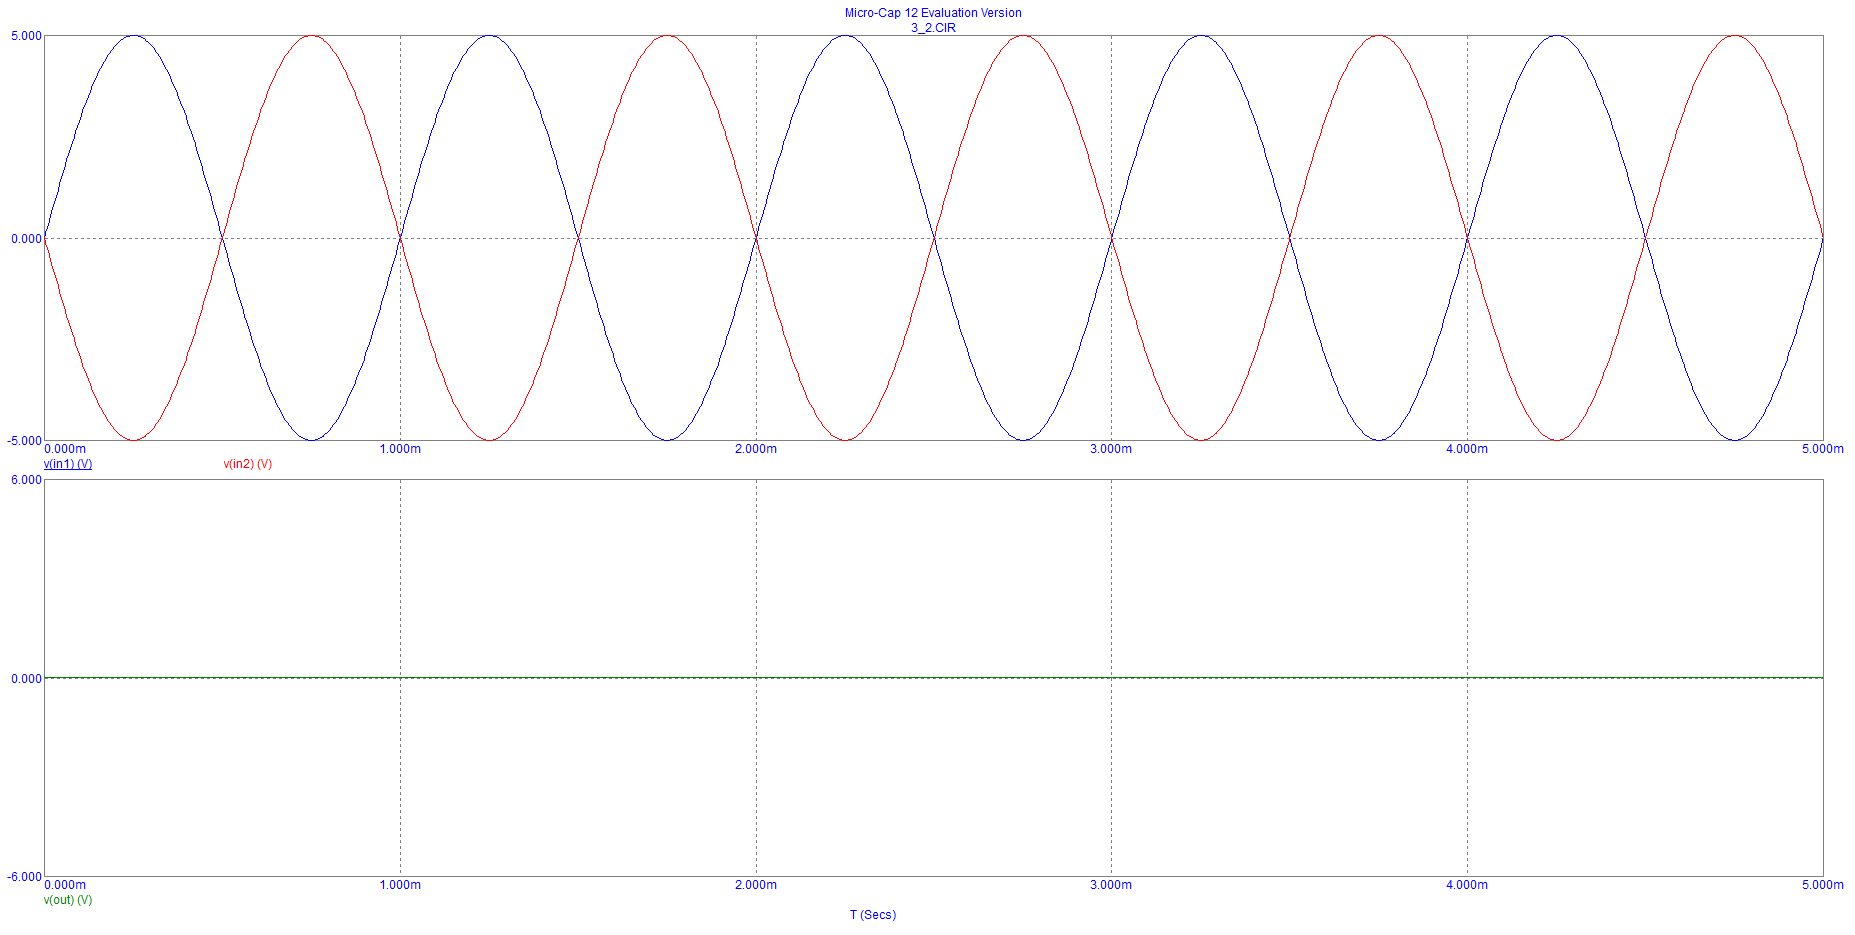
\includegraphics[width=\textwidth]{PC/ukol2/nula_vzstup.png}
    Časový průběh se dvěma vstupními signály lišící se vzájemným posunutím \(180^\circ\) \(U_{pp} = 10\-[V]\) \(f = 1\-[kHz]\).
  \end{minipage}
\end{figure}

\begin{figure}[H]
  \begin{minipage}[t]{0.48\textwidth}
    \centering
    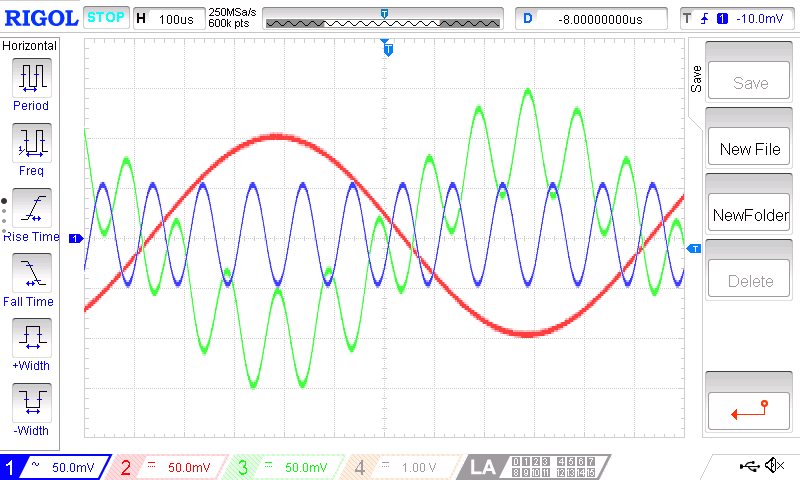
\includegraphics[width=\textwidth]{LAB/NewFile3.png}
    Změřený časový průběh dvou různých signálů sumačním zesilovače a jeho výstup. \\
    signál-1 \(U_{pp} = 200\-[mV]\) \(f = 1\-[kHz]\) \\
    signál-2 \(U_{pp} = 100\-[mV]\) \(f = 10\-[kHz]\).
  \end{minipage}
  \hfill
  \begin{minipage}[t]{0.48\textwidth}
    \centering
    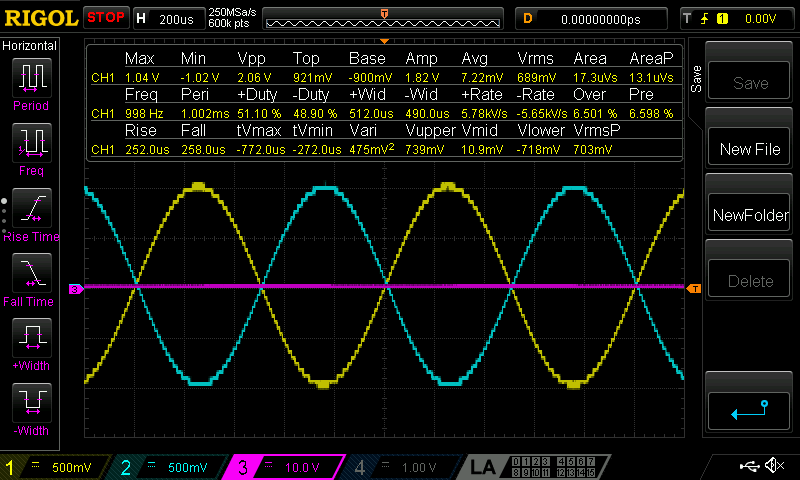
\includegraphics[width=\textwidth]{LAB/NewFile6.png}
    Změřený časový průběh se dvěma vstupními signály lišící se vzájemným posunutím \(180^\circ\) \(U_{pp} = 2\-[V]\) \(f = 1\-[kHz]\).
  \end{minipage}
\end{figure}

\subsection*{Diferenční zesilovač}
\begin{figure}[H]
  \begin{minipage}[t]{\textwidth}
    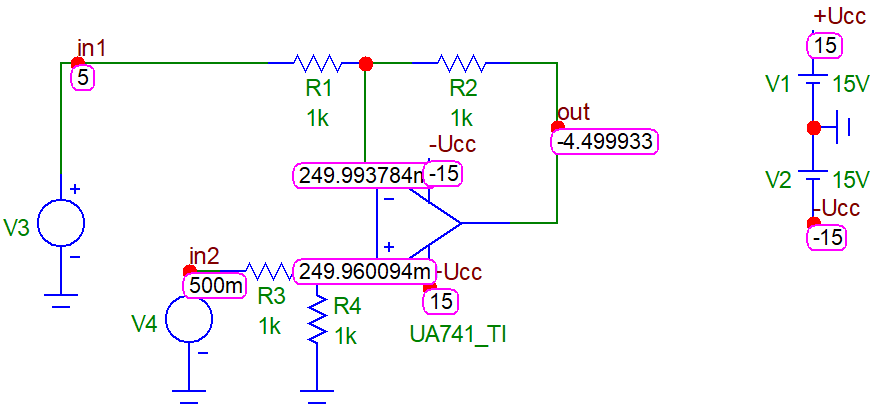
\includegraphics[width=\textwidth]{PC/ukol3/DC.png}
  \end{minipage}
\end{figure}

\begin{figure}[H]
  \begin{minipage}[t]{\textwidth}
    \centering
    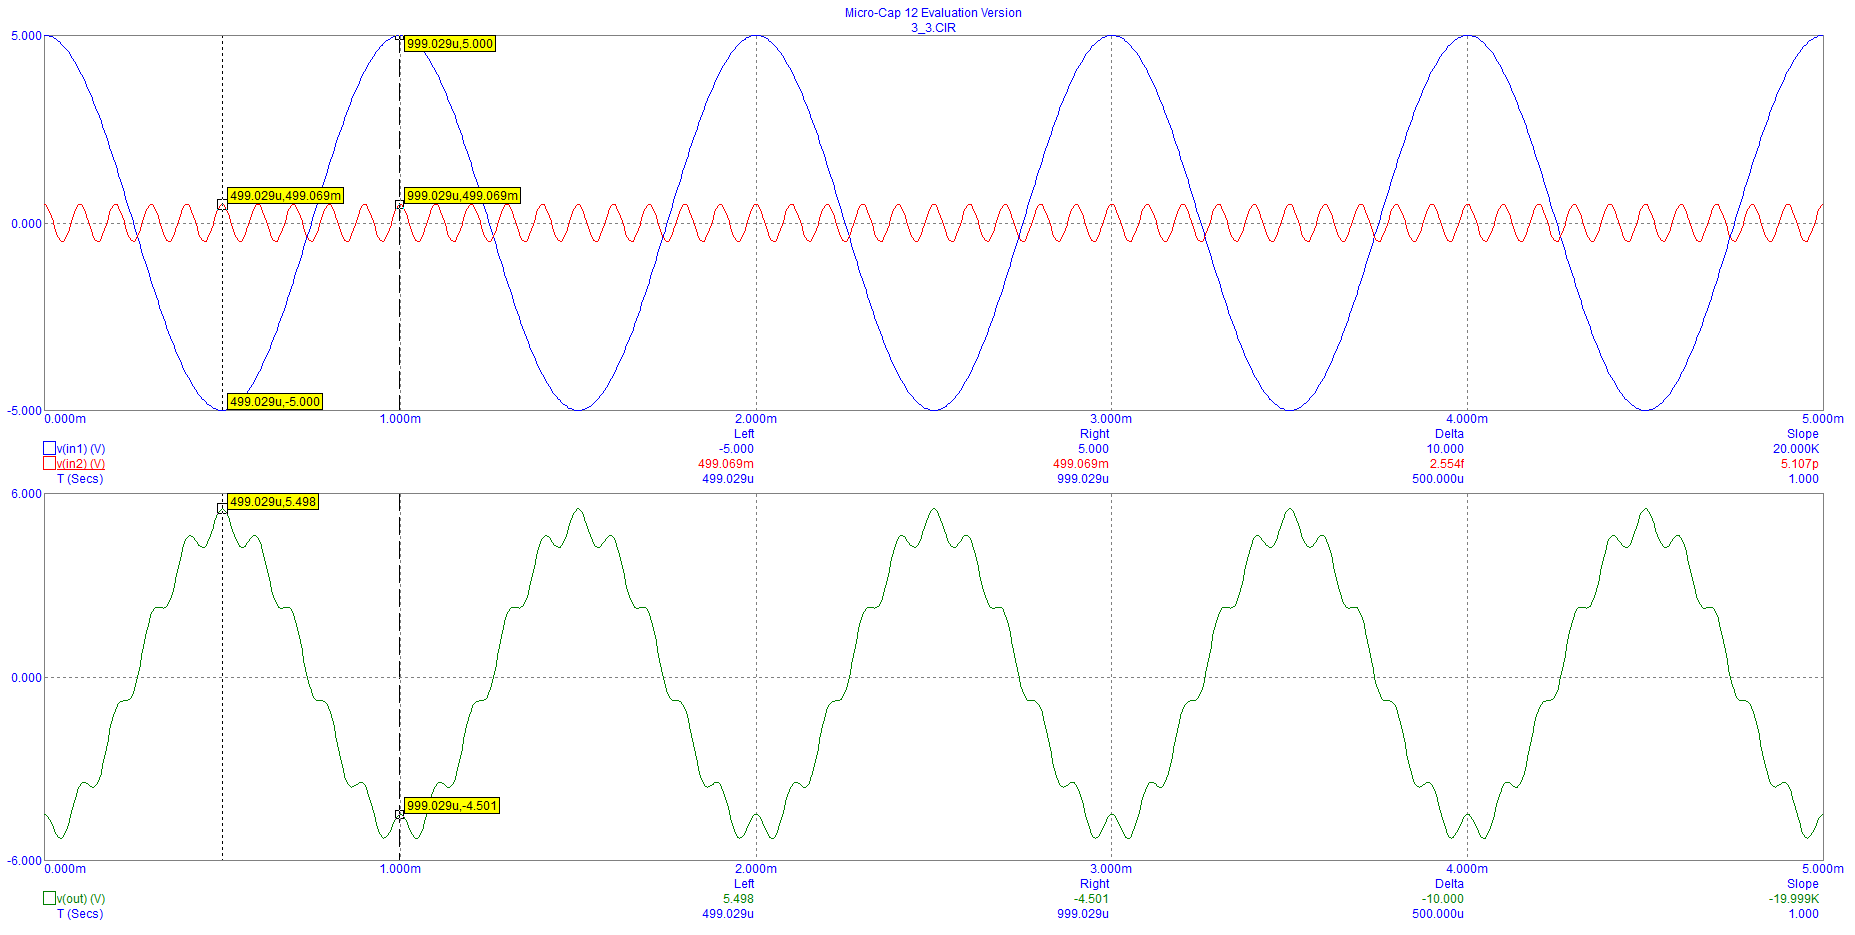
\includegraphics[width=\textwidth]{PC/ukol3/transient4.png}
    Časový průběh se dvěma rozdílnými vstupními signály \\
    signál-1 \(U_{pp} = 10\-[V]\) \(f = 1\-[kHz]\) \\
    signál-2 \(U_{pp} = 1\-[V]\) \(f = 10\-[kHz]\).
  \end{minipage}
\end{figure}

\begin{figure}[H]
  \begin{minipage}[t]{\textwidth}
    \centering
    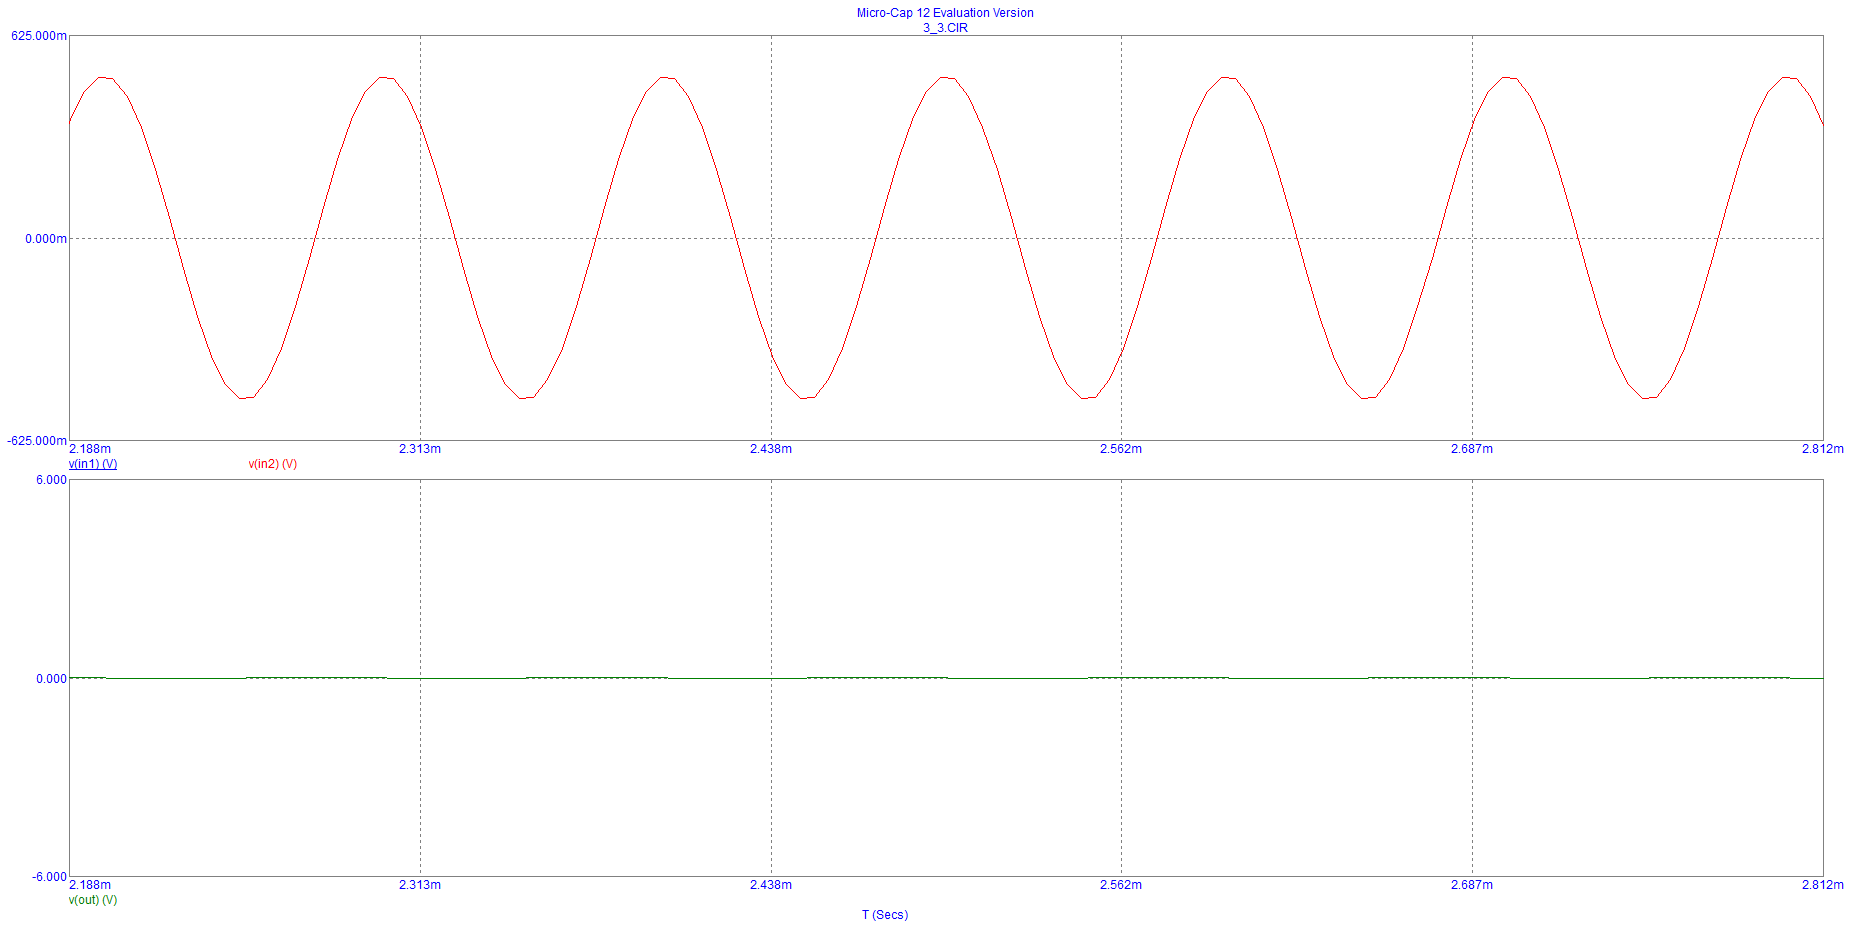
\includegraphics[width=\textwidth]{PC/ukol3/nula_vzstup.png}
    Časový průběh se dvěma identickými vstupními signály \(U_{pp} = 10\-[V]\) \(f = 1\-[kHz]\).
  \end{minipage}
\end{figure}

\begin{figure}[H]
  \begin{minipage}[t]{0.48\textwidth}
    \centering
    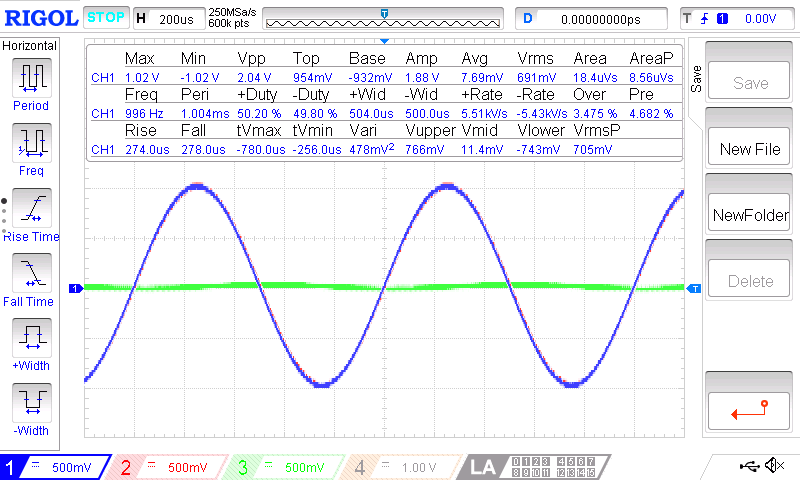
\includegraphics[width=\textwidth]{LAB/NewFile8.png}
    Změřený časový průběh se dvěma identickými vstupními signály \(U_{pp} = 2\-[V]\) \(f = 1\-[kHz]\).
  \end{minipage}
  \hfill
  \begin{minipage}[t]{0.48\textwidth}
    \centering
    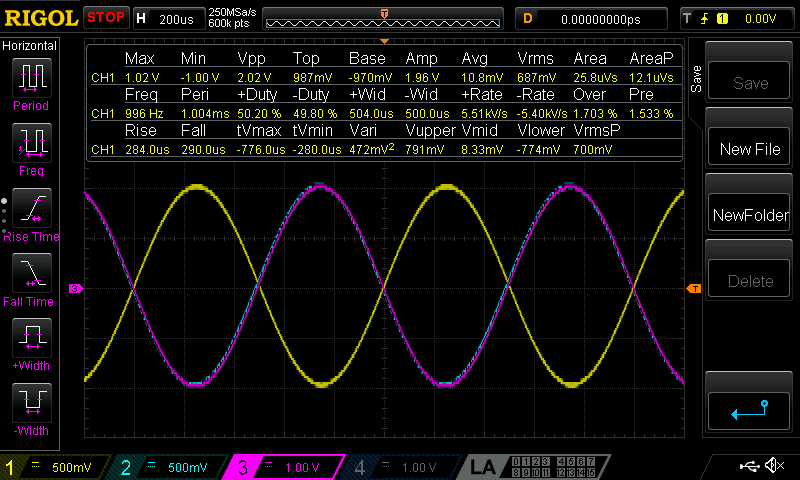
\includegraphics[width=\textwidth]{LAB/NewFile9.png}
    Změřený časový průběh se dvěma vstupními signály lišící se vzájemným posunutím \(180^\circ\) \(U_{pp} = 2\-[V]\) \(f = 1\-[kHz]\).
  \end{minipage}
\end{figure}
\begin{figure}[H]
  \begin{minipage}[t]{\textwidth}
    \centering
    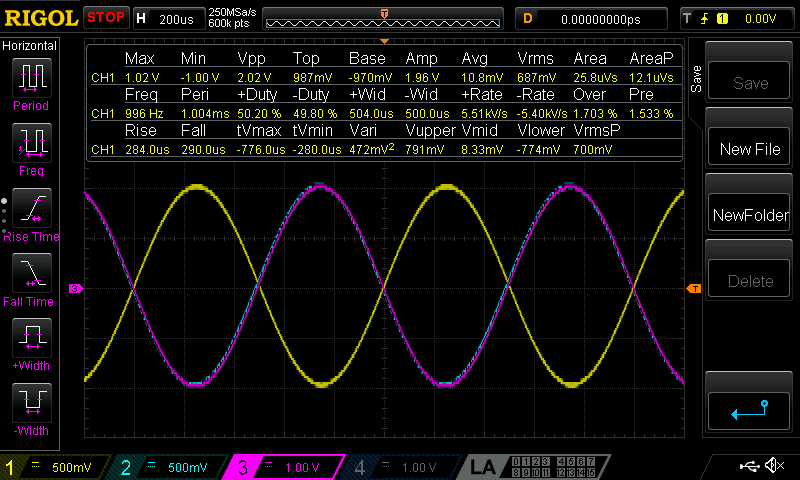
\includegraphics[width=\textwidth]{LAB/NewFile9.png}
    Časový průběh se dvěma rozdílnými vstupními signály \\
    signál-1 \(U_{pp} = 2\-[V]\) \(f = 1\-[kHz]\) \\
    signál-2 \(U_{pp} = 200\-[mV]\) \(f = 10\-[kHz]\).
  \end{minipage}
\end{figure}

\newpage
\subsection{Závěr}

Z prvního zapojení je vidět, že se OZ dá použít i jen s jedním zdrojem napájení, při vytvoření referenčního napájení.
Pokud v dalším zapojení vadí takto vytvořená stejnosměrná složka, dá se vstup a výstup oddělit kapacitorem.

Další zapojení ukazuje, jak sečíst dva signály do jednoho.
Poslední zapojení ukazuje, jak od sebe dva signály odečíst.
Měření i simulace ukazují, co se stane s výstupním signálem, když na vstup přivedeme dva stejné, různé a vzájemně opačné signály pro obě dvě zapojení.

Měření všech tří reálných zapojení, i jejich simulace, odpovídá teorii z numerických cvičení.
U druhého zapojení je důležité si povšimnout, že vstupní signály sice sečte, ale výsledek následně invertuje, jak je vidět na následujícím obrázku.
\begin{figure}[H]
  \begin{minipage}[t]{\textwidth}
    \centering
    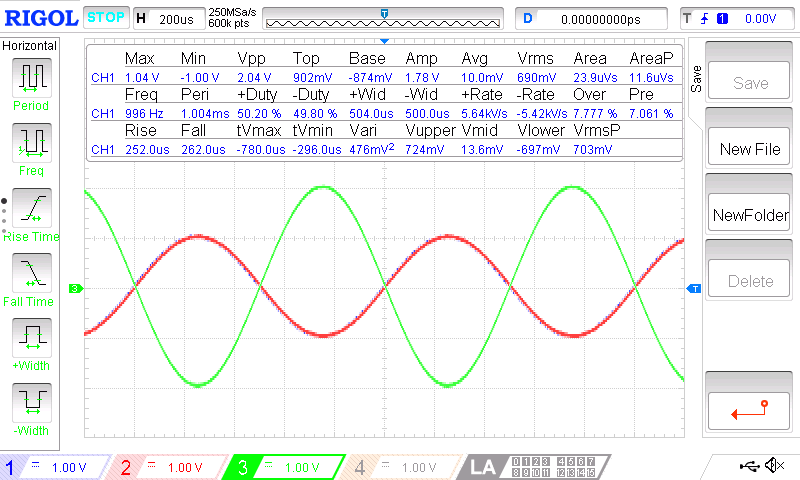
\includegraphics[width=\textwidth]{LAB/NewFile7.png}
    Časový průběh se dvěma identickými vstupními signály \(U_{pp} = 2\-[V]\) \(f = 1\-[kHz]\).
  \end{minipage}
\end{figure}

Z teorie také plyne, že jak sumační, tak diferenční zesilovač může krom prostého sčítání resp. odčítání signálu jednotlivé složky násobit.
Tato funkce je v našich zapojeních ovlivněna všemi rezistory, z čehož také plynou nadstandardní požadavky na přesnost těchto rezistorů.

Oproti tomu zapojení zesilovače s nesymetrickým napájením má vysoké požadavky na přesnost rezistoru \(R_1\) a \(R_2\) zatím co u \(R_3\) a \(R_4\) ne až tolik.
Nepřesnost rezistoru \(R_3\) a \(R_4\) by způsobila různé saturační napětí v kladném a záporném směru, nikoliv však zkreslení signálu v okolí střední hodnoty.
Proto na rezistory \(R_3\) a \(R_4\) nejsou tak vysoké požadavky jako \(R_1\) a \(R_2\).

\begin{table}[H]
  \centering
  \begin{tabular}{|c|c|c|c|c|c|c|} 
    \hline
    uzel \(n\)          & 1       & 2      & 3     & 4     & 5       & 6      \\ \hline
    NC \(U_{nG}\-[V]\)  & 15      & 7.5    & 7.5   & 7.5   & 7.5     & 0      \\ \hline
    PC \(U_{nG}\-[V]\)  & 15      & 7.499  & 7.499 & 7.499 & 7.499   & 0      \\ \hline
    LC \(U_{nG}\-[V]\)  & 15.074  & 7.536  & 7.539 & 7.536 & 7.537   & 0      \\ \hline

  \end{tabular}
  \normalsize
  \caption{Porovnání výsledku stejnosměrné analýzy z NC, PC a LC}
\end{table}

\end{document}
